\section{Conceptual Model and Simulation Design }

\subsection{Derivation from system analysis}

The conceptual model is directly derived from the process analysis made in section 1. The system boundary is defined as the AMC clinic session, spanning from patient arrival to exit after checkout. The private practice is not explicitly modeled but serves as a reference baseline in the qualitative analysis. The flow unit is the individual patient, who carries a type attribute assigned at the generation and used to determine routing throughout the model. 

\subsection{Process representation}

The process flow is shown in \autoref{fig:FlowChart} in the appendix, developed as a flowchart based on the process design tools in chapter 4 \parencite[p. 118-120]{pensumbok}. All patients enter through a common intake path before being routed to one of the three paths based on patient type. New and Return patients follow the full AMC clinical path. This is Resident Review, Resident and Patient, Teach and Resident and Attending before proceeding to check-out. Follow-up patients are routed to the PA, after which a probabilistic branch determines whether an in-person consultation is required before check-out. 

\begin{figure}[H]
    \centering
    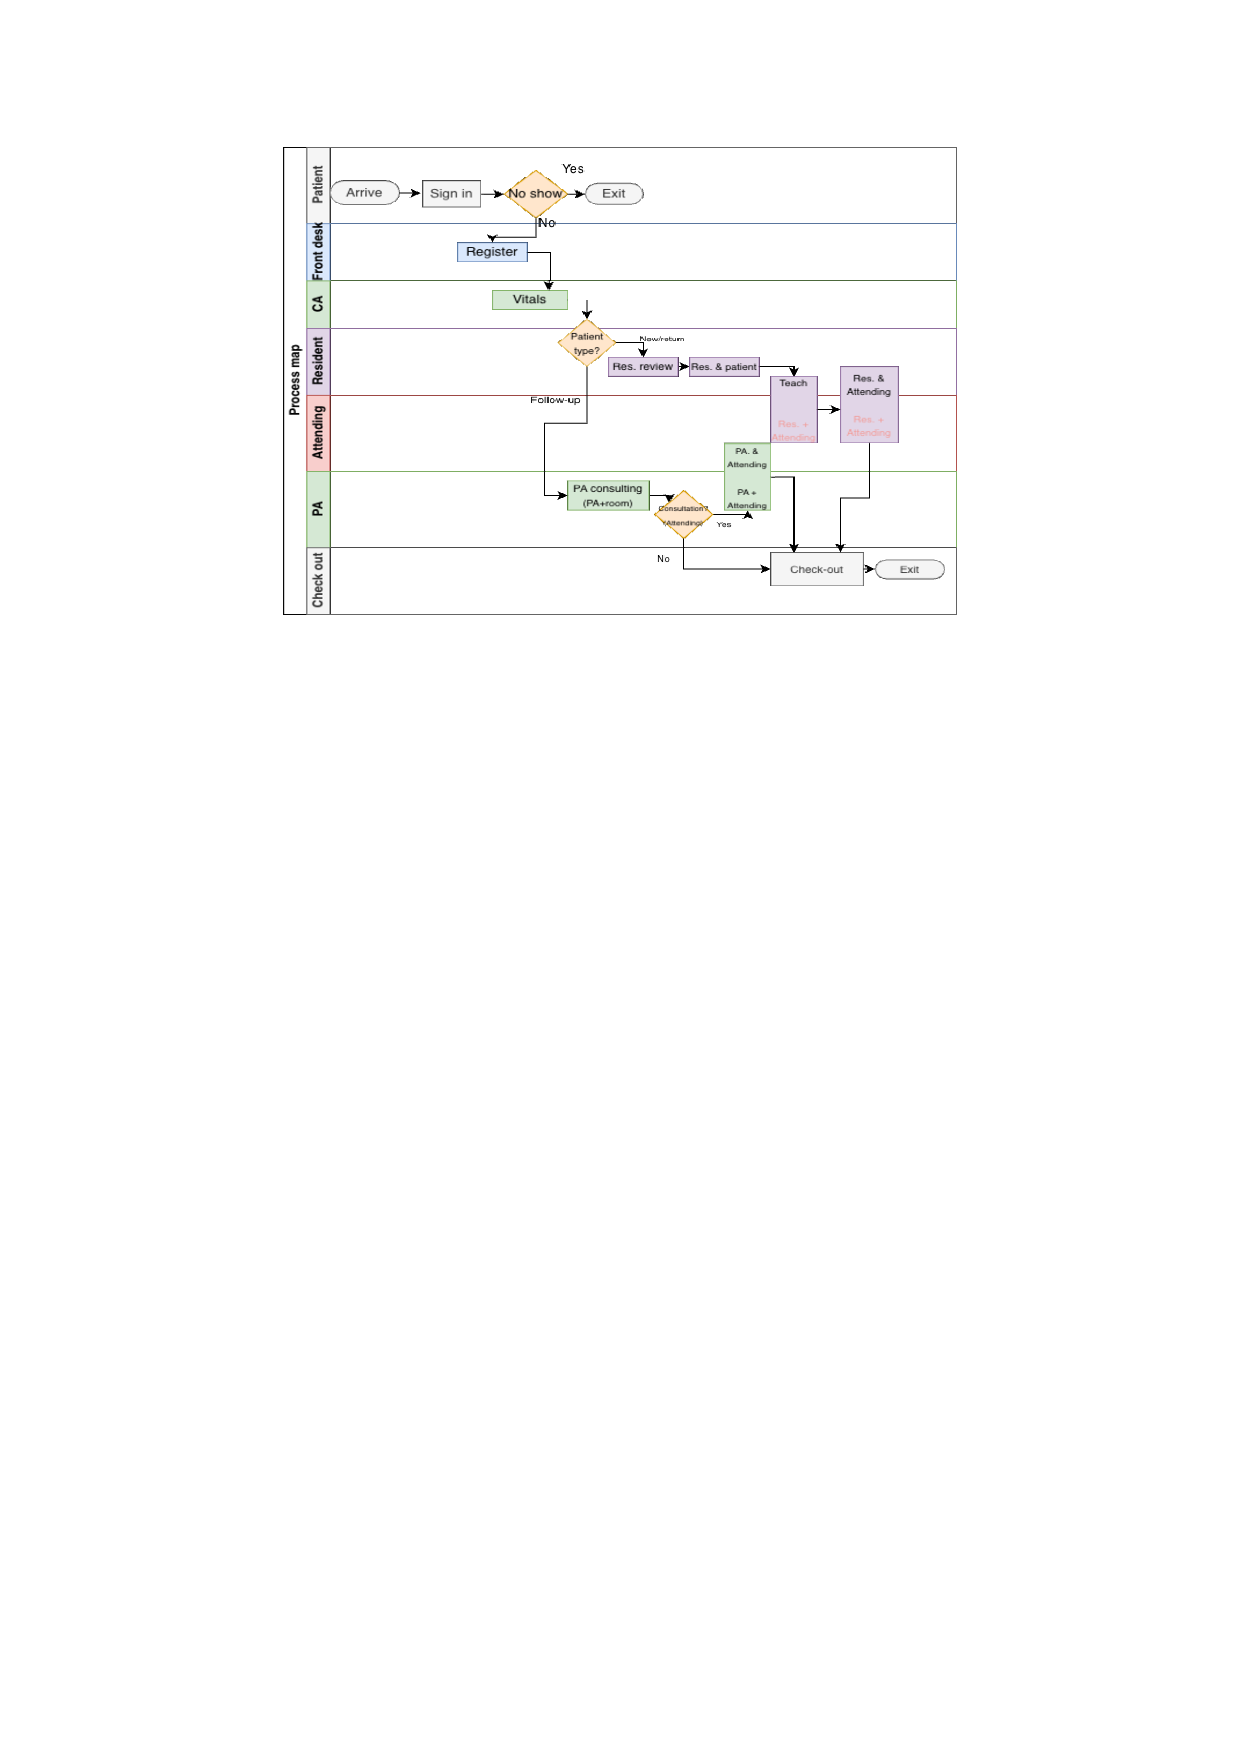
\includegraphics[width=0.4\textwidth]{Inputs/Pictures/Figure2.pdf}
    \caption{Process map}
    \label{fig:ProcessMap}
\end{figure}

A decision point for no-show patients is modelled after Sign In, with a 10\% probability of exit. This reflects the case description that 10\% of scheduled appointments are cancelled, and that the clinic learns of these cancellations too late to fill the slot, meaning the appointment time is lost but no service is used. Arrivals are not modelled as a stochastic process, instead patients are generated according to the fixed schedule template shown in Table 6 of the case \parencite[Table 6]{MillerPainTreatmentCenter}. 

\subsection{Modelling assumptions}

Several simplifying assumptions are made to make the model manageable. First, Sign in is modelled as instantaneous, as it represents a time stamp event rather than a service activity consuming staff time. Second, the three residents are modelled as a shared resource pool with capacity 3 rather than as individually tracked agents. The patient entity seizes a resident from the pool at Resident Review and holds the resource through the entire sequence until Resident and Attending is complete. This reflects the case description that each resident follows a single patient through the full interaction. Third, teaching time variability across attending physicians is not modelled explicitly, a single fitted distribution is used for the Teach step representing an average across physicians. Fourth, the PA examination room is modeled as a separate resource from the three rooms used for New and Return patients, and as consistent with the case we note that the PA's room is not available for other types of visits.

\subsection{Mapping to JaamSim}

The mapping from conceptual components to JaamSim implementation is summarized in Table 2 found in the appendix. Each activity is implemented as Server object. Routing decisions are implemented as Branch objects. A Queue object precedes each Server, with first in first out priority discipline. Routing decisions are implemented as Branch objects, and deterministic appointment arrivals are implemented using an EventSchedule object linked to an EntityGenerator. Patients who do not show up exit through an EntitySink after the no-show branch, while patients completing Check-out exit through the same sink via a Statistic object that records total time in system. 

Four resources are implemented as Resource objects. Resource acquisition and release are handled through Seize and release objects. For new and return patients, a resident and an exam room are seized before Resident Review and held through Resident and Attending is complete. The Attending is seized before Teach and released only after Resident and Attending, ensuring it cannot be simultaneously engaged in more than one activity, directly reflecting the bottleneck identified in section 3.1a. For Follow-up patients, the PA exam room is seized before the PA step, and the Attending is seized for only 50\% of cases requiring a consultation. 